\documentclass[10pt]{book}
\usepackage[
  paperwidth=5.5in,
  paperheight=8.5in,
  inner=0.5in, % Margin on the binding side
  outer=0.75in,% Margin on the outside edge
  top=.75in,
  bottom=.75in,
  twoside  % Enables mirroring of inner/outer margins
]{geometry}
\usepackage{setspace}
\usepackage{lmodern}
\usepackage{parskip}
\usepackage{titlesec}
\usepackage{titling}
\usepackage{graphicx}
\usepackage{etoolbox}
\usepackage{fancyhdr}
\usepackage{ebgaramond}
\usepackage{calc}
\usepackage{changepage} % in preamble
\usepackage{verse}
\usepackage{adjustbox}

\newcommand{\idt}{\hspace*{1em}}

\newenvironment{poemblock}{}{}

%MACRO FOR POEM CHAPTER 
\newcommand{\poemchapter}[1]{%
  \def\poemtitle{#1}
  \section*{\poemtitle}
  \markboth{\poemtitle}{\poemtitle}
  \addcontentsline{toc}{section}{\poemtitle}
}


%MACRO FOR INDENTED BLOCK:
%usage:  \indentedblock\itshape{}
\newcommand{\indentedblock}[2]{
  \begin{adjustwidth}{2em}{0pt}
{\setlength{\parindent}{0pt}
 #1 % styling command like \itshape
 #2 % the actual content
}
  \end{adjustwidth}
}

%MACRO FOR INDENTED BLOCK WITH NO SECOND SHAPING
\newcommand{\indentedblockns}[1]{
  \begin{adjustwidth}{2em}{0pt}
{\setlength{\parindent}{0pt}
 #1 
}
  \end{adjustwidth}%
}

\setlength{\headheight}{15pt}
\addtolength{\topmargin}{-3pt}

% Header/Footer style
\pagestyle{fancy}
\fancyhf{}
\fancyhead[LE,RO]{\thepage}
\fancyhead[RE]{\leftmark}
\fancyhead[LO]{\rightmark}

% Prevent chapter headings from adding "Chapter" prefix
\titleformat{\chapter}[display]
  {\normalfont\LARGE\bfseries\centering}{}{0pt}{}

% Begin Document
\begin{document}

\thispagestyle{empty}
\null
\newpage

\thispagestyle{empty}
\null
\newpage

% Title Page
\begin{titlepage}
\centering
{\Huge\bfseries Ballads of A Cheechako\par}
{\Huge\bfseries \&\par}
{\Huge\bfseries Songs of a Sourdough\par}
\vspace{2em}

\begin{figure}[htbp]
  \centering
  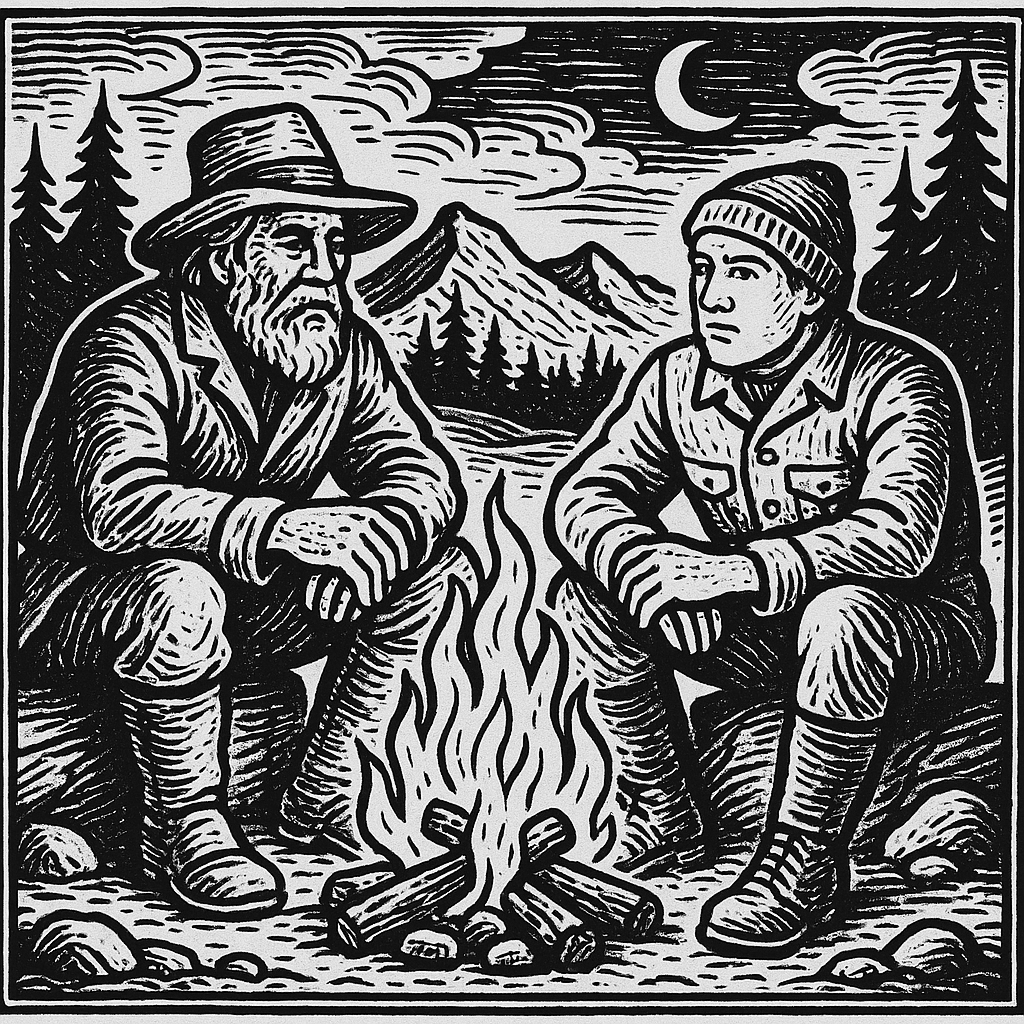
\includegraphics[width=0.5\textwidth]{images/fireside}
\end{figure}

{\Huge Robert W. Service\par}


\vspace{10em}
{\large Modernized edition by Arthur Strutzenberg, 2025\par}
{\large Originally Published by William Briggs, Toronto\par}
{\large 1907 and 1909}
\end{titlepage}

\newpage
\thispagestyle{empty}
\null
\newpage

\frontmatter
\tableofcontents
\newpage

\mainmatter
%\cleardoublepage
\chapter*{Foreword}
\addcontentsline{toc}{chapter}{Foreword}
\markboth{}{}
\vspace{1em}

I first discovered the poetry of Robert W. Service one night as a child, when my mother read to me from a weathered collection of his verse. I still remember her voice as she launched into “\textit{The Cremation of Sam McGee}” — the firelight flickering in the room, the strange comfort of that icy tale, and the rhythm that made it feel like both a story and a song.

Later that same night, she read me “\textit{Grin},” and something in its message stayed with me — a rough, resilient courage wrapped in rhyme. Though time passed and the words faded, I recently stumbled across the poem again, and the memory of that moment returned with clarity.

This book is, in part, a tribute to that night and to the enduring voice of the man known as the Bard of the Yukon. His poems have a way of cutting through the years — bold, humorous, unflinching — and reminding us that even in the face of hardship, we can press on... and perhaps even grin.



% Actual Poems
\cleardoublepage
\chapter*{Ballads of A Cheechako}
\addcontentsline{toc}{chapter}{Ballads of a Cheechako}
\poemchapter{To the Man of the High North}

\begin{poemblock}
My rhymes are rough, and often in my rhyming\\
\idt I've drifted, silver-sailed, on seas of dream,\\
Hearing afar the bells of Elfland chiming,\\
\idt Seeing the groves of Arcadie agleam.

I was the thrall of Beauty that rejoices\\
\idt From peak snow-diademed to regal star;\\
Yet to mine aerie ever pierced the voices,\\
\idt The pregnant voices of the Things That Are.

The Here, the Now, the vast Forlorn around us;\\
\idt The gold-delirium, the ferine strife;\\
The lusts that lure us on, the hates that hound us;\\
\idt Our red rags in the patch-work quilt of Life.

The nameless men who nameless rivers travel,\\
\idt And in strange valleys greet strange deaths alone;\\
\idt The grim, intrepid ones who would unravel\\
The mysteries that shroud the Polar Zone.

These will I sing, and if one of you linger\\
\idt Over my pages in the Long, Long Night,\\
And on some lone line lay a calloused finger,\\
\idt Saying:  "It's human-true--it hits me right";\\
Then will I count this loving toil well spent;\\
Then will I dream awhile--content, content.
\end{poemblock}

\newpage


\cleardoublepage
\chapter*{Songs of a Sourdough}
\addcontentsline{toc}{chapter}{Songs of a Sourdough}
\poemchapter{The Law of the Yukon}

\begin{adjustwidth}{0em}{0em}
\begin{poemblock}
This is the law of the Yukon, and ever she makes it plain:\\
"Send not your foolish and feeble; send me your strong and your sane.\\
Strong for the red rage of battle; sane, for I harry them sore;\\
Send me men girt for the combat, men who are grit to the core;\\
Swift as the panther in triumph, fierce as the bear in defeat,\\
Sired of a bulldog parent, steeled in the furnace heat.\\
Send me the best of your breeding, lend me your chosen ones;\\
Them will I take to my bosom, them will I call my sons;\\
Them will I gild with my treasure, them will I glut with my meat;\\
But the others—the misfits, the failures—I trample under my feet.\\
Dissolute, damned, and despairful, crippled and palsied and slain,\\
Ye would send me the spawn of your gutters—Go! take back your spawn again.

"Wild and wide are my borders, stern as death is my sway;\\
From my ruthless throne I have ruled alone for a million years and a day;\\
Hugging my mighty treasure, waiting for man to come:\\
Till he swept like a turbid torrent, and after him swept—the scum.\\
The pallid pimp of the dead-line, the enervate of the pen,\\
One by one I weeded them out, for all that I sought was—Men.\\
One by one I dismayed them, frighting them sore with my glooms;\\
One by one I betrayed them unto my manifold dooms.\\
Drowned them like rats in my rivers, starved them like curs on my plains,\\
Rotted the flesh that was left them, poisoned the blood in their veins;\\
Burst with my winter upon them, searing forever their sight,\\
Lashed them with fungus-white faces, whimpering wild in the night;\\
Staggering blind through the storm-whirl, stumbling mad through the snow,\\
Frozen stiff in the ice pack, brittle and bent like a bow;\\
Featureless, formless, forsaken, scented by wolves in their flight,\\
Left for the wind to make music through ribs that are glittering white;\\
Gnawing the black crust of failure, searching the pit of despair,\\
Crooking the toe in the trigger, trying to patter a prayer;\\
Going outside with an escort, raving with lips all afoam;\\
Writing a cheque for a million, drivelling feebly of home;\\
Lost like a louse in the burning ... or else in tented town\\
Seeking a drunkard's solace, sinking and sinking down;\\
Steeped in the slime at the bottom, dead to a decent world,\\
Lost 'mid the human flotsam, far on the frontier hurled;\\
In the camp at the bend of the river, with its dozen saloons aglare,\\
Its gambling dens a-riot, its gramophones all a-blare;\\
Crimped with the crimes of a city, sin-ridden and bridled with lies,\\
In the hush of my mountained vastness, in the flush of my midnight skies.\\
Plague-spots, yet tools of my purpose, so natheless I suffer them thrive,\\
Crushing my Weak in their clutches, that only my Strong may survive.

"But the others, the men of my mettle, the men who would 'stablish my fame,\\
Unto its ultimate issue, winning me honour, not shame;\\
Searching my uttermost valleys, fighting each step as they go,\\
Shooting the wrath of my rapids, scaling my ramparts of snow;\\
Ripping the guts of my mountains, looting the beds of my creeks,\\
Them will I take to my bosom, and speak as a mother speaks.\\
I am the land that listens, I am the land that broods;\\
Steeped in eternal beauty, crystalline waters and woods.\\
Long have I waited lonely, shunned as a thing accurst,\\
Monstrous, moody, pathetic, the last of the lands and the first;\\
Visioning camp-fires at twilight, sad with a longing forlorn,\\
Feeling my womb o'er-pregnant with the seed of cities unborn.\\
Wild and wide are my borders, stern as death is my sway,\\
And I wait for the men who will win me—and I will not be won in a day;\\
And I will not be won by weaklings, subtile, suave, and mild,\\
But by men with the hearts of vikings, and the simple faith of a child;\\
Desperate, strong, and resistless, unthrottled by fear or defeat,\\
Them will I gild with my treasure, them will I glut with my meat.

"Lofty I stand from each sister land, patient and wearily wise,\\
With the weight of a world of sadness in my quiet, passionless eyes;\\
Dreaming alone of a people, dreaming alone of a day,\\
When men shall not rape my riches, and curse me and go away;\\
Making a bawd of my bounty, fouling the hand that gave—\\
Till I rise in my wrath and I sweep on their path and I stamp them into a grave.\\
Dreaming of men who will bless me, of women esteeming me good,\\
Of children born in my borders, of radiant motherhood;\\
Of cities leaping to stature, of fame like a flag unfurled,\\
As I pour the tide of my riches in the eager lap of the world."

This is the Law of the Yukon, that only the Strong shall thrive;\\
That surely the Weak shall perish, and only the Fit survive.\\
Dissolute, damned, and despairful, crippled and palsied and slain,\\
This is the Will of the Yukon,—Lo! how she makes it plain!\\
\end{poemblock}
\end{adjustwidth}

\newpage
\poemchapter{The Parson's Son}


\begin{poemblock}
\textit{
This is the song of the parson's son, as he squats in his shack alone,\\
On the wild, weird nights when the Northern Lights shoot up from the frozen zone,\\
And it's sixty below, and couched in the snow the hungry huskies moan.
}

"I'm one of the Arctic brotherhood, I'm an old-time pioneer.\\
I came with the first—O God! how I've cursed this Yukon—but still I'm here.\\
I've sweated athirst in its summer heat, I've frozen and starved in its cold;\\
I've followed my dreams by its thousand streams, I've toiled and moiled for its gold.

"Look at my eyes—been snow-blind twice; look where my foot's half gone;\\
And that gruesome scar on my left cheek where the frost-fiend bit to the bone.\\
Each one a brand of this devil's land, where I've played and I've lost the game,\\
A broken wreck with a craze for 'hooch,' and never a cent to my name.

"This mining is only a gamble, the worst is as good as the best;\\
I was in with the bunch and I might have come out right on top with the rest;\\
With Cormack, Ladue and Macdonald—O God! but it's hell to think\\
Of the thousands and thousands I've squandered on cards and women and drink.

"In the early days we were just a few, and we hunted and fished around,\\
Nor dreamt by our lonely camp-fires of the wealth that lay under the ground.\\
We traded in skins and whiskey, and I've often slept under the shade\\
Of that lone birch-tree on Bonanza, where the first big find was made.

"We were just like a great big family, and every man had his squaw,\\
And we lived such a wild, free, fearless life beyond the pale of the law;\\
Till sudden there came a whisper, and it maddened us every man,\\
And I got in on Bonanza before the big rush began.

"Oh, those Dawson days, and the sin and the blaze, and the town all open wide!\\
(If God made me in His likeness, sure He let the devil inside.)\\
But we all were mad, both the good and the bad, and as for the women, well—\\
No spot on the map in so short a space has hustled more souls to hell.

"Money was just like dirt there, easy to get and to spend.\\
I was all caked in on a dance-hall jade, but she shook me in the end.\\
It put me queer, and for near a year I never drew sober breath,\\
Till I found myself in the bughouse ward with a claim staked out on death.

"Twenty years in the Yukon, struggling along its creeks;\\
Roaming its giant valleys, scaling its god-like peaks;\\
Bathed in its fiery sunsets, fighting its fiendish cold,\\
Twenty years in the Yukon ... twenty years—and I'm old.

"Old and weak, but no matter, there's 'hooch' in the bottle still.\\
I'll hitch up the dogs to-morrow, and mush down the trail to Bill.\\
It's so long dark, and I'm lonesome—I'll just lay down on the bed,\\
To-morrow I'll go ... to-morrow ... I guess I'll play on the red.

"... Come, Kit, your pony is saddled. I'm waiting, dear, in the court ...\\
...Minnie, you devil, I'll kill you if you skip with that flossy sport ...\\
... How much does it go to the pan, Bill?... play up, School, and play the game ...\\
... Our Father, which art in heaven, hallowed be Thy name ..."

\textit{
This was the song of the parson's son, as he lay in his bunk alone,
Ere the fire went out and the cold crept in, and his blue lips ceased to moan,
And the hunger-maddened malamutes had torn him flesh from bone.
}

\end{poemblock}

\newpage
\poemchapter{The Spell of the Yukon}

\begin{poemblock}
I wanted the gold, and I sought it;\\
\idt I scrabbled and mucked like a slave.\\
Was it famine or scurvy—I fought it,\\
\idt I hurled my youth into the grave.\\
I wanted the gold and I got it—\\
\idt Came out with a fortune last fall,—\\
Yet somehow life's not what I thought it,\\
\idt And somehow the gold isn't all.

No! There's the land. (Have you seen it?)\\
\idt It's the cussedest land that I know,\\
From the big, dizzy mountains that screen it,\\
\idt To the deep, deathlike valleys below.\\
Some say God was tired when He made it;\\
\idt Some say it's a fine land to shun;\\
Maybe: but there's some as would trade it\\
\idt For no land on earth—and I'm one.

You come to get rich (damned good reason),\\
\idt You feel like an exile at first;\\
You hate it like hell for a season,\\
\idt And then you are worse than the worst.\\
It grips you like some kinds of sinning;\\
\idt It twists you from foe to a friend;\\
It seems it's been since the beginning;\\
\idt It seems it will be to the end.

I've stood in some mighty-mouthed hollow\\
\idt That's plumb-full of hush to the brim;\\
I've watched the big, husky sun wallow\\
\idt In crimson and gold, and grow dim,\\
Till the moon set the pearly peaks gleaming,\\
\idt And the stars tumbled out, neck and crop;\\
And I've thought that I surely was dreaming,\\
\idt With the peace o' the world piled on top.

The summer—no sweeter was ever;\\
\idt The sunshiny woods all athrill;\\
The grayling aleap in the river,\\
\idt The bighorn asleep on the hill.\\
The strong life that never knows harness;\\
\idt The wilds where the caribou call;\\
The freshness, the freedom, the farness—\\
\idt O God! how I'm stuck on it all.

The winter! the brightness that blinds you,\\
\idt The white land locked tight as a drum,\\
The cold fear that follows and finds you,\\
\idt The silence that bludgeons you dumb.\\
The snows that are older than history,\\
\idt The woods where the weird shadows slant;\\
The stillness, the moonlight, the mystery,\\
\idt I've bade 'em good-bye—but I can't.

There's a land where the mountains are nameless,\\
\idt And the rivers all run God knows where;\\
There are lives that are erring and aimless,\\
\idt And deaths that just hang by a hair;\\
There are hardships that nobody reckons;\\
\idt There are valleys unpeopled and still;\\
There's a land—oh, it beckons and beckons,\\
\idt And I want to go back—and I will.

They're making my money diminish;\\
\idt I'm sick of the taste of champagne.\\
Thank God! when I'm skinned to a finish\\
\idt I'll pike to the Yukon again.\\
I'll fight—and you bet it's no sham-fight;\\
\idt It's hell!—but I've been there before;\\
And it's better than this by a damsite—\\
\idt So me for the Yukon once more.

There's gold, and it's haunting and haunting;\\
\idt It's luring me on as of old;\\
Yet it isn't the gold that I'm wanting,\\
\idt So much as just finding the gold.\\
It's the great, big, broad land 'way up yonder,\\
\idt It's the forests where silence has lease;\\
It's the beauty that thrills me with wonder,\\
\idt It's the stillness that fills me with peace.

\end{poemblock}

\newpage
\poemchapter{TITLE HERE}


\begin{verse}
VERSE\\
VERSE\\
VERSE
\end{verse}

\newpage
\poemchapter{The Lone Trail}

\begin{poemblock}
\textit{
Ye who know the Lone Trail fain would follow it,\\
\idt Though it lead to glory or the darkness of the pit.\\
Ye who take the Lone Trail, bid your love good-bye;\\
\idt The Lone Trail, the Lone Trail follow till you die.
}

The trails of the world be countless, and most of the trails be tried;\\
\idt You tread on the heels of the many, till you come where the ways divide;\\
And one lies safe in the sunlight, and the other is dreary and wan,\\
\idt Yet you look aslant at the Lone Trail, and the Lone Trail lures you on.\\
And somehow you're sick of the highway, with its noise and its easy needs,\\
\idt And you seek the risk of the by-way, and you reck not where it leads.\\
And sometimes it leads to the desert, and the tongue swells out of the mouth,\\
\idt And you stagger blind to the mirage, to die in the mocking drouth.\\
And sometimes it leads to the mountain, to the light of the lone camp-fire,\\
\idt And you gnaw your belt in the anguish of hunger-goaded desire.\\
And sometimes it leads to the Southland, to the swamp where the orchid glows,\\
\idt And you rave to your grave with the fever, and they rob the corpse for its clothes.\\
And sometimes it leads to the Northland, and the scurvy softens your bones,\\
\idt And your flesh dints in like putty, and you spit out your teeth like stones.\\
And sometimes it leads to a coral reef in the wash of a weedy sea,\\
\idt And you sit and stare at the empty glare where the gulls wait greedily.\\
And sometimes it leads to an Arctic trail, and the snows where your torn feet freeze,\\
\idt And you whittle away the useless clay, and crawl on your hands and knees.\\
Often it leads to the dead-pit; always it leads to pain;\\
\idt By the bones of your brothers ye know it, but oh, to follow you're fain.\\
By your bones they will follow behind you, till the ways of the world are made plain.

\textit{
Bid good-bye to sweetheart, bid good-bye to friend;\\
\idt The Lone Trail, the Lone Trail follow to the end.\\
Tarry not, and fear not, chosen of the true;\\
\idt Lover of the Lone Trail, the Lone Trail waits for you.
}
\end{poemblock}

\newpage
\poemchapter{TITLE HERE}


\begin{verse}
VERSE\\
VERSE\\
VERSE
\end{verse}

\newpage
\poemchapter{The Three Voices}

\begin{poemblock}
The waves have a story to tell me,\\
\idt As I lie on the lonely beach;\\
Chanting aloft in the pine-tops,\\
\idt The wind has a lesson to teach;\\
But the stars sing an anthem of glory\\
\idt I cannot put into speech.

The waves tell of ocean spaces,\\
\idt Of hearts that are wild and brave,\\
Of populous city places,\\
\idt Of desolate shores they lave;\\
Of men who sally in quest of gold\\
\idt To sink in an ocean grave.

The wind is a mighty roamer;\\
\idt He bids me keep me free,\\
Clean from the taint of the gold-lust,\\
\idt Hardy and pure as he;\\
Cling with my love to nature\\
\idt As a child to the mother-knee.

But the stars throng out in their glory,\\
\idt And they sing of the God in man;\\
They sing of the mighty Master,\\
\idt Of the loom His fingers span;\\
Where a star or a soul is a part of the whole,\\
\idt And weft in the wondrous plan.

Here by the camp-fire's flicker,\\
\idt Deep in my blanket curled,\\
I long for the peace of the pine-gloom\\
\idt When the scroll of the Lord is unfurled,\\
And the wind and the wave are silent,\\
\idt And world is singing to world.

\end{poemblock}

\newpage
\poemchapter{TITLE HERE}


\begin{verse}
VERSE\\
VERSE\\
VERSE
\end{verse}

\newpage
\poemchapter{The Harpy}


\begin{poemblock}
\textit{
There was a woman, and she was wise; woefully wise was she;\\
She was old, so old, yet her years all told were but a score and three;\\
And she knew by heart, from finish to start, the Book of Iniquity.
}

There is no hope for such as I, on earth nor yet in Heaven;\\
Unloved I live, unloved I die, unpitied, unforgiven;\\
A loathèd jade I ply my trade, unhallowed and unshriven.

I paint my cheeks, for they are white, and cheeks of chalk men hate;\\
Mine eyes with wine I make to shine, that men may seek and sate;\\
With overhead a lamp of red I sit me down and wait.

Until they come, the nightly scum, with drunken eyes aflame;\\
Your sweethearts, sons, ye scornful ones—'tis I who know their shame;\\
The gods ye see are brutes to me—and so I play my game.

For life is not the thing we thought, and not the thing we plan;\\
And woman in a bitter world must do the best she can;\\
Must yield the stroke, and bear the yoke, and serve the will of man;

Must serve his need and ever feed the flame of his desire;\\
Though be she loved for love alone, or be she loved for hire;\\
For every man since life began is tainted with the mire.

And though you know he love you so, and set you on love's throne,\\
Yet let your eyes but mock his sighs, and let your heart be stone,\\
Lest you be left (as I was left) attainted and alone.

From love's close kiss to hell's abyss is one sheer flight, I trow;\\
And wedding-ring and bridal bell are will-o'-wisps of woe;\\
And 'tis not wise to love too well, and this all women know.

Wherefore, the wolf-pack having gorged upon the lamb, their prey,\\
With siren smile and serpent guile I make the wolf-pack pay;\\
With velvet paws and flensing claws, a tigress roused to slay.

One who in youth sought truest truth, and found a devil's lies;\\
A symbol of the sin of man, a human sacrifice:\\
Yet shall I blame on man the shame? Could it be otherwise?

Was I not born to walk in scorn where others walk in pride?\\
The Maker marred, and evil-starred I drift upon His tide;\\
And He alone shall judge His own, so I His judgment bide.

\textit{
Fate has written a tragedy; its name is "The Human Heart."\\
The theatre is the House of Life, Woman the mummer's part:\\
The Devil enters the prompter's box and the play is ready to start.
}
\end{poemblock}

\newpage
\poemchapter{TITLE HERE}


\begin{verse}
VERSE\\
VERSE\\
VERSE
\end{verse}

\newpage
\poemchapter{The Song of the Wage-Slave}


\begin{verse}
When the long, long day is over, and the Big Boss gives me my pay,\\
I hope that it won't be hell-fire, as some of the parsons say.\\
And I hope that it won't be heaven, with some of the parsons I've met—\\
All I want is just quiet, just to rest and forget.\\
Look at my face, toil-furrowed; look at my calloused hands;\\
Master, I've done Thy bidding, wrought in Thy many lands—\\
Wrought for the little masters, big-bellied they be, and rich;\\
I've done their desire for a daily hire, and I die like a dog in a ditch.\\
I have used the strength Thou hast given, Thou knowest I did not shirk;\\
Threescore years of labour—Thine be the long day's work.\\
And now, Big Master, I'm broken and bent and twisted and scarred,\\
But I've held my job, and Thou knowest, and Thou wilt not judge me hard.\\
Thou knowest my sins are many, and often I've played the fool—\\
Whiskey and cards and women, they made me the devil's tool.\\
I was just like a child with money: I flung it away with a curse,\\
Feasting a fawning parasite, or glutting a harlot's purse,\\
Then back to the woods repentant, back to the mill or the mine,\\
I, the worker of workers, everything in my line.\\
Everything hard but headwork (I'd no more brains than a kid),\\
A brute with brute strength to labour, doing as I was bid;\\
Living in camps with men-folk, a lonely and loveless life;\\
Never knew kiss of sweetheart, never caress of wife.\\
A brute with brute strength to labour, and they were so far above—\\
Yet I'd gladly have gone to the gallows for one little look of Love.\\
I with the strength of two men, savage and shy and wild—\\
Yet how I'd ha' treasured a woman, and the sweet, warm kiss of a child.\\
Well, 'tis Thy world, and Thou knowest. I blaspheme and my ways be rude;\\
But I've lived my life as I found it, and I've done my best to be good;\\
I, the primitive toiler, half naked, and grimed to the eyes,\\
Sweating it deep in their ditches, swining it stark in their styes,\\
Hulling down forests before me, spanning tumultuous streams;\\
Down in the ditch building o'er me palaces fairer than dreams;\\
Boring the rock to the ore-bed, driving the road through the fen,\\
Resolute, dumb, uncomplaining, a man in a world of men.\\
Master, I've filled my contract, wrought in Thy many lands;\\
Not by my sins wilt Thou judge me, but by the work of my hands.\\
Master, I've done Thy bidding, and the light is low in the west,\\
And the long, long shift is over ... Master, I've earned it—Rest. 
\end{verse}

\newpage
\input{poems/SongsOfASourdough/grin}
\newpage
\poemchapter{TITLE HERE}


\begin{verse}
VERSE\\
VERSE\\
VERSE
\end{verse}

\newpage
\poemchapter{The Cremation of Sam McGee}

\begin{verse}
\textit{
There are strange things done in the midnight sun\\
\hspace*{2em}By the men who moil for gold;\\
The Arctic trails have their secret tales\\
\hspace*{2em}That would make your blood run cold;\\
The Northern Lights have seen queer sights,\\
\hspace*{2em}But the queerest they ever did see\\
Was that night on the marge of Lake Lebarge\\
\hspace*{2em}I cremated Sam McGee.
}

Now Sam McGee was from Tennessee,\\
\hspace*{2em}Where the cotton blooms and blows.\\
Why he left his home in the South to roam\\
\hspace*{2em}‘Round the Pole, God only knows.\\
He was always cold, but the land of gold\\
\hspace*{2em}Seemed to hold him like a spell;\\
Though he’d often say in his homely way\\
\hspace*{2em}That “he’d sooner live in hell.”

On a Christmas Day we were mushing our way\\
\hspace*{2em}Over the Dawson trail.\\
Talk of your cold!—through the parka’s fold\\
\hspace*{2em}It stabbed like a driven nail.\\
If our eyes we’d close, then the lashes froze\\
\hspace*{2em}Till sometimes we couldn’t see;\\
It wasn’t much fun, but the only one\\
\hspace*{2em}To whimper was Sam McGee.

And that very night, as we lay packed tight\\
\hspace*{2em}In our robes beneath the snow,\\
And the dogs were fed, and the stars o’erhead\\
\hspace*{2em}Were dancing heel and toe,\\
He turned to me, and “Cap,” says he,\\
\hspace*{2em}“I’ll cash in this trip, I guess;\\
And if I do, I’m asking that you\\
\hspace*{2em}Won’t refuse my last request.”

Well, he seemed so low that I couldn’t say no;\\
\hspace*{2em}Then he says with a sort of moan:\\
“It’s the cursed cold, and it’s got right hold\\
\hspace*{2em}Till I’m chilled clean through to the bone.\\
Yet ‘tain’t being dead—it’s my awful dread\\
\hspace*{2em}Of the icy grave that pains;\\
So I want you to swear that, foul or fair,\\
\hspace*{2em}You’ll cremate my last remains.”

A pal’s last need is a thing to heed,\\
\hspace*{2em}So I swore I would not fail;\\
And we started on at the streak of dawn,\\
\hspace*{2em}But God! he looked ghastly pale.\\
He crouched on the sleigh, and he raved all day\\
\hspace*{2em}Of his home in Tennessee;\\
And before nightfall a corpse was all\\
\hspace*{2em}That was left of Sam McGee.

There wasn’t a breath in that land of death,\\
\hspace*{2em}And I hurried, horror-driven,\\
With a corpse half hid that I couldn’t get rid,\\
\hspace*{2em}Because of a promise given;\\
It was lashed to the sleigh, and it seemed to say:\\
\hspace*{2em}“You may tax your brawn and brains,\\
But you promised true, and it’s up to you\\
\hspace*{2em}To cremate those last remains.”

Now a promise made is a debt unpaid,\\
\hspace*{2em}And the trail has its own stern code.\\
In the days to come, though my lips were dumb,\\
\hspace*{2em}In my heart how I cursed that load.\\
In the long, long night, by the lone firelight,\\
\hspace*{2em}While the huskies, round in a ring,\\
Howled out their woes to the homeless snows—\\
\hspace*{2em}O God! how I loathed the thing.

And every day that quiet clay\\
\hspace*{2em}Seemed to heavy and heavier grow;\\
And on I went, though the dogs were spent\\
\hspace*{2em}And the grub was getting low;\\
The trail was bad, and I felt half mad,\\
\hspace*{2em}But I swore I would not give in;\\
And I’d often sing to the hateful thing,\\
\hspace*{2em}And it hearkened with a grin.

Till I came to the marge of Lake Lebarge,\\
\hspace*{2em}And a derelict there lay;\\
It was jammed in the ice, but I saw in a trice\\
\hspace*{2em}It was called the “Alice May.”\\
And I looked at it, and I thought a bit,\\
\hspace*{2em}And I looked at my frozen chum;\\
Then “Here,” said I, with a sudden cry,\\
\hspace*{2em}“Is my crematorium.”

Some planks I tore from the cabin floor,\\
\hspace*{2em}And I lit the boiler fire;\\
Some coal I found that was lying around,\\
\hspace*{3em}And I heaped the fuel higher;\\
The flames just soared, and the furnace roared—\\
\hspace*{2em}Such a blaze you seldom see;\\
And I burrowed a hole in the glowing coal,\\
\hspace*{2em}And I stuffed in Sam McGee.

Then I made a hike, for I didn’t like\\
\hspace*{2em}To hear him sizzle so;\\
And the heavens scowled, and the huskies howled,\\
\hspace*{2em}And the wind began to blow.\\
It was icy cold, but the hot sweat rolled\\
\hspace*{2em}Down my cheeks, and I don’t know why;\\
And the greasy smoke in an inky cloak\\
\hspace*{2em}Went streaking down the sky.

I do not know how long in the snow\\
\hspace*{2em}I wrestled with grisly fear;\\
But the stars came out and they danced about\\
\hspace*{2em}Ere again I ventured near;\\
I was sick with dread, but I bravely said:\\
\hspace*{2em}“I’ll just take a peep inside.\\
I guess he’s cooked, and it’s time I looked.”\\
\hspace*{2em}... Then the door I opened wide.

And there sat Sam, looking cool and calm,\\
\hspace*{2em}In the heart of the furnace roar;\\
And he wore a smile you could see a mile,\\
\hspace*{2em}And he said: “Please close that door.\\
It’s fine in here, but I greatly fear\\
\hspace*{2em}You’ll let in the cold and storm—\\
Since I left Plumtree, down in Tennessee,\\
\hspace*{2em}It’s the first time I’ve been warm.”

\textit{
There are strange things done in the midnight sun\\
\hspace*{2em}By the men who moil for gold;\\
The Arctic trails have their secret tales\\
\hspace*{2em}That would make your blood run cold;\\
The Northern Lights have seen queer sights,\\
\hspace*{2em}But the queerest they ever did see\\
Was that night on the marge of Lake Lebarge\\
\hspace*{2em}I cremated Sam McGee.
}

\end{verse}

\newpage
\poemchapter{TITLE HERE}


\begin{verse}
VERSE\\
VERSE\\
VERSE
\end{verse}

\newpage
\poemchapter{TITLE HERE}


\begin{verse}
VERSE\\
VERSE\\
VERSE
\end{verse}

\newpage
\poemchapter{TITLE HERE}


\begin{verse}
VERSE\\
VERSE\\
VERSE
\end{verse}

\newpage
\poemchapter{TITLE HERE}


\begin{verse}
VERSE\\
VERSE\\
VERSE
\end{verse}

\newpage
\poemchapter{TITLE HERE}


\begin{verse}
VERSE\\
VERSE\\
VERSE
\end{verse}

\newpage
\poemchapter{Music in the Bush}

\begin{poemblock}
O'er the dark pines she sees the silver moon,\\
\idt And in the west, all tremulous, a star;\\
And soothing sweet she hears the mellow tune\\
\idt Of cow-bells jangled in the fields afar.

Quite listless, for her daily stent is done,\\
\idt She stands, sad exile, at her rose-wreathed door,\\
And sends her love eternal with the sun\\
\idt That goes to gild the land she'll see no more.

The grave, gaunt pines imprison her sad gaze,\\
\idt All still the sky and darkling drearily;\\
She feels the chilly breath of dear, dead days\\
\idt Come sifting through the alders eerily.

Oh, how the roses riot in their bloom!\\
\idt The curtains stir as with an ancient pain;\\
Her old piano gleams from out the gloom,\\
\idt And waits and waits her tender touch in vain.

But now her hands like moonlight brush the keys\\
\idt With velvet grace, melodious delight;\\
And now a sad refrain from overseas\\
\idt Goes sobbing on the bosom of the night.

And now she sings. (O singer in the gloom,\\
\idt Voicing a sorrow we can ne'er express,\\
Here in the Farness where we few have room\\
\idt Unshamed to show our love and tenderness,

Our hearts will echo, till they beat no more,\\
\idt That song of sadness and of motherland;\\
And stretched in deathless love to England's shore,\\
\idt Some day she'll hearken and she'll understand.)

A prima-donna in the shining past,\\
\idt But now a mother growing old and grey,\\
She thinks of how she held a people fast\\
\idt In thrall, and gleaned the triumphs of a day.

She sees a sea of faces like a dream;\\
\idt She sees herself a queen of song once more;\\
She sees lips part in rapture, eyes agleam;\\
\idt She sings as never once she sang before.

She sings a wild, sweet song that throbs with pain,\\
\idt The added pain of life that transcends art,\\
A song of home, a deep, celestial strain,\\
\idt The glorious swan-song of a dying heart.

A lame tramp comes along the railway track,\\
\idt A grizzled dog whose day is nearly done:\\
He passes, pauses, then comes slowly back\\
\idt And listens there—an audience of one.

She sings—her golden voice is passion-fraught\\
\idt As when she charmed a thousand eager ears;\\
He listens trembling, and she knows it not,\\
\idt And down his hollow cheeks roll bitter tears.

She ceases and is still, as if to pray;\\
\idt There is no sound, the stars are all alight—\\
Only a wretch who stumbles on his way,\\
\idt Only a vagrant sobbing in the night.

\end{poemblock}

\newpage
\poemchapter{The Rhyme of the Remittance Man}

\begin{poemblock}
There's a four-pronged buck a-swinging in the shadow of my cabin,\\
\idt And it roamed the velvet valley till to-day;\\
But I tracked it by the river, and I trailed it in the cover,\\
\idt And I killed it on the mountain miles away.\\
Now I've had my lazy supper, and the level sun is gleaming\\
\idt On the water where the silver salmon play;\\
And I light my little corn-cob, and I linger softly dreaming,\\
\idt \idt In the twilight, of a land that's far away.

Far away, so faint and far, is flaming London, fevered Paris,\\
\idt That I fancy I have gained another star;\\
Far away the din and hurry, far away the sin and worry,\\
\idt Far away—God knows they cannot be too far.\\
Gilded galley-slaves of Mammon—how my purse-proud brothers taunt me!\\
\idt I might have been as well-to-do as they\\
Had I clutched like them my chances, learned their wisdom, crushed my fancies,\\
\idt Starved my soul and gone to business every day.

Well, the cherry bends with blossom, and the vivid grass is springing,\\
\idt And the star-like lily nestles in the green;\\
And the frogs their joys are singing, and my heart in tune is ringing,\\
\idt And it doesn't matter what I might have been,\\
While above the scented pine-gloom, piling heights of golden glory,\\
\idt The sun-god paints his canvas in the west;\\
I can couch me deep in clover, I can listen to the story\\
\idt Of the lazy, lapping water—it is best.

While the trout leaps in the river, and the blue grouse thrills the cover,\\
\idt And the frozen snow betrays the panther's track,\\
And the robin greets the dayspring with the rapture of a lover,\\
\idt I am happy, and I'll nevermore go back. \\
For I know I'd just be longing for the little old log cabin,\\
\idt With the morning-glory clinging to the door,\\
Till I loathed the city places, cursed the care on all the faces,\\
\idt Turned my back on lazar London evermore.

So send me far from Lombard Street, and write me down a failure;\\
\idt Put a little in my purse and leave me free.\\
Say: "He turned from Fortune's offering to follow up a pale lure,\\
\idt He is one of us no longer—let him be."\\
I am one of you no longer: by the trails my feet have broken,\\
\idt The dizzy peaks I've scaled, the camp-fire's glow,\\
By the lonely seas I've sailed in—yea, the final word is spoken,\\
\idt I am signed and sealed to nature. Be it so.
\end{poemblock}

\newpage
\poemchapter{TITLE HERE}


\begin{verse}
VERSE\\
VERSE\\
VERSE
\end{verse}

\newpage
\poemchapter{TITLE HERE}


\begin{verse}
VERSE\\
VERSE\\
VERSE
\end{verse}

\newpage
\poemchapter{TITLE HERE}


\begin{verse}
VERSE\\
VERSE\\
VERSE
\end{verse}

\newpage
\poemchapter{The March of the Dead}

\begin{poemblock}
The cruel war was over—oh, the triumph was so sweet!\\
\idt We watched the troops returning, through our tears;\\
There was triumph, triumph, triumph down the scarlet glittering street,\\
\idt And you scarce could hear the music for the cheers.\\
And you scarce could see the house-tops for the flags that flew between,\\
\idt The bells were pealing madly to the sky;\\
And every one was shouting for the Soldiers of the Queen,\\
\idt And the glory of an age was passing by.

And then there came a shadow, swift and sudden, dark and drear;\\
\idt The bells were silent, not an echo stirred.\\
The flags were drooping sullenly, the men forgot to cheer;\\
\idt We waited, and we never spoke a word.\\
The sky grew darker, darker, till from out the gloomy rack\\
\idt There came a voice that checked the heart with dread:\\
"Tear down, tear down your bunting now, and hang up sable black;\\
\idt They are coming—it's the Army of the Dead."

They were coming, they were coming, gaunt and ghastly, sad and slow;\\
\idt They were coming, all the crimson wrecks of pride;\\
With faces seared, and cheeks red smeared, and haunting eyes of woe,\\
\idt And clotted holes the khaki couldn't hide.\\
Oh, the clammy brow of anguish! the livid, foam-flecked lips!\\
\idt The reeling ranks of ruin swept along!\\
The limb that trailed, the hand that failed, the bloody finger-tips!\\
\idt And oh, the dreary rhythm of their song!

"They left us on the veldt-side, but we felt we couldn't stop,\\
\idt On this, our England's crowning festal day;\\
We're the men of Magersfontein, we're the men of Spion Kop,\\
\idt Colenso,—we're the men who had to pay.\\
We're the men who paid the blood-price. Shall the grave be all our gain?\\
\idt You owe us. Long and heavy is the score.\\
Then cheer us for our glory now, and cheer us for our pain,\\
\idt And cheer us as ye never cheered before."

The folks were white and stricken, and each tongue seemed weighed with lead;\\
\idt Each heart was clutched in hollow hand of ice;\\
And every eye was staring at the horror of the dead,\\
\idt The pity of the men who paid the price.\\
They were come, were come to mock us, in the first flush of our peace;\\
\idt Through writhing lips their teeth were all agleam;\\
They were coming in their thousands—oh, would they never cease!\\
\idt I closed my eyes, and then—it was a dream.

There was triumph, triumph, triumph down the scarlet gleaming street;\\
\idt The town was mad, a man was like a boy.\\
A thousand flags were flaming where the sky and city meet;\\
\idt A thousand bells were thundering the joy.\\
There was music, mirth and sunshine; but some eyes shone with regret:\\
\idt And while we stun with cheers our homing braves,\\
O God, in Thy great mercy, let us nevermore forget\\
\idt The graves they left behind, the bitter graves.

\end{poemblock}

\newpage
\poemchapter{TITLE HERE}


\begin{verse}
VERSE\\
VERSE\\
VERSE
\end{verse}

\newpage
\poemchapter{The Woman And The Angel}


\begin{verse}
An angel was tired of heaven, as he lounged in the golden street;\\
His halo was tilted sideways, and his harp lay mute at his feet;\\
So the Master stooped in His pity, and gave him a pass to go,\\
For the space of a moon, to the earth-world, to mix with the men below.

He doffed his celestial garments, scarce waiting to lay them straight;\\
He bade goodbye to Peter, who stood by the golden gate;\\
The sexless singers of heaven chanted a fond farewell,\\
And the imps looked up as they pattered on the red-hot flags of hell.

Never was seen such an angel: eyes of a heavenly blue,\\
Features that shamed Apollo, hair of a golden hue;\\
The women simply adored him, his lips were like Cupid's bow;\\
But he never ventured to use them—and so they voted him slow.

Till at last there came One Woman, a marvel of loveliness,\\
And she whispered to him: "Do you love me?" And he answered that woman, "Yes."\\
And she said: "Put your arms around me, and kiss me, and hold me—so—"\\
But fiercely he drew back, saying: "This thing is wrong, and I know."

Then sweetly she mocked his scruples, and softly she him beguiled:\\
"You, who are verily man among men, speak with the tongue of a child.\\
We have outlived the old standards; we have burst, like an over-tight thong,\\
The ancient, outworn, puritanic traditions of Right and Wrong."

Then the Master feared for His angel, and called him again to His side,\\
For oh, the woman was wondrous, and oh, the angel was tried.\\
And deep in his hell sang the Devil, and this was the strain of his song:\\
"The ancient, outworn, puritanic traditions of Right and Wrong."

\end{verse}

\newpage
\poemchapter{The Rhyme of the Restless Ones}


\begin{poemblock}
We couldn't sit and study for the law;\\
\idt The stagnation of a bank we couldn't stand;\\
For our riot blood was surging, and we didn't need much urging\\
To excitements and excesses that are banned.\\
So we took to wine and drink and other things,\\
\idt And the devil in us struggled to be free;\\
Till our friends rose up in wrath, and they pointed out the path,\\
And they paid our debts and packed us o'er the sea.

Oh, they shook us off and shipped us o'er the foam,\\
To the larger lands that lure a man to roam;\\
\idt And we took the chance they gave\\
\idt Of a far and foreign grave,\\
And we bade goodbye for evermore to home.

And some of us are climbing on the peak,\\
\idt And some of us are camping on the plain;\\
By pine and palm you'll find us, with never claim to bind us,\\
By track and trail you'll meet us once again.

We are fated serfs to freedom—sky and sea;\\
\idt We have failed where slummy cities overflow;\\
But the stranger ways of earth know our pride and know our worth,\\
And we go into the dark as fighters go.

Yes, we go into the night as brave men go,\\
Though our faces they be often streaked with woe;\\
\idt Yet we're hard as cats to kill,\\
\idt And our hearts are reckless still,\\
And we've danced with death a dozen times or so.

And you'll find us in Alaska after gold,\\
\idt And you'll find us herding cattle in the South.\\
We like strong drink and fun; and when the race is run,\\
\idt We often die with curses in our mouth.

We are wild as colts unbroke, but never mean;\\
\idt Of our sins we've shoulders broad to bear the blame;\\
But we'll never stay in town, and we'll never settle down,\\
\idt And we'll never have an object or an aim.

No, there's that in us that time can never tame;\\
And life will always seem a careless game;\\
\idt And they'd better far forget—\\
\idt Those who say they love us yet—\\
Forget, blot out with bitterness our name.

\end{poemblock}

\newpage
\poemchapter{TITLE HERE}


\begin{verse}
VERSE\\
VERSE\\
VERSE
\end{verse}

\newpage
\poemchapter{Comfort}


\begin{verse}
Say! You've struck a heap of trouble—\\
\hspace*{3em}Bust in business, lost your wife;\\
No one cares a cent about you,\\
\hspace*{3em}You don't care a cent for life;\\
Hard luck has of hope bereft you,\\
\hspace*{3em}Health is failing, wish you'd die—\\
Why, you've still the sunshine left you,\\
\hspace*{3em}And the big, blue sky.

\hspace*{6em}Sky so blue it makes you wonder\\
\hspace*{9em}If it's heaven shining through;\\
\hspace*{6em}Earth so smiling 'way out yonder,\\
\hspace*{9em}Sun so bright it dazzles you;\\
\hspace*{6em}Birds a-singing, flowers a-flinging\\
\hspace*{9em}All their fragrance on the breeze;\\
\hspace*{6em}Dancing shadows, green, still meadows—\\
\hspace*{9em}Don't you mope, you've still got these.

These, and none can take them from you;\\
\hspace*{3em}These, and none can weigh their worth.\\
What! you're tired and broke and beaten?—\\
\hspace*{3em}Why, you're rich—you've got the earth!\\
Yes, if you're a tramp in tatters,\\
\hspace*{3em}While the blue sky bends above,\\
You've got nearly all that matters,\\
\hspace*{3em}You've got God, and God is love.

\end{verse}

\newpage
\poemchapter{TITLE HERE}


\begin{verse}
VERSE\\
VERSE\\
VERSE
\end{verse}

\newpage
\poemchapter{TITLE HERE}


\begin{verse}
VERSE\\
VERSE\\
VERSE
\end{verse}

\newpage
\poemchapter{L'Envoi}


\begin{verse}

\textit{
You who have lived in the Land,\\
\idt You who have trusted the trail;\\
You who are strong to withstand,\\
\idt You who are swift to assail;\\
Songs have I sung to beguile,\\
\idt Vintage of desperate years\\
Hard as a harlot's smile,\\
\idt Bitter as unshed tears.
}

\indentedblock\itshape{
Little of joy or mirth,\\
\idt Little of ease I sing;\\
Sagas of men of earth,\\
\idt Humanly suffering,\\
Such as you all have done;\\
\idt Savagely faring forth,\\
Sons of the midnight sun,\\
\idt Argonauts of the North.
}

\textit{
Far in the land God forgot\\
\idt Glimmers the lure of your trail;\\
Still in your lust are you taught\\
\idt Even to win is to fail.\\
Still must you follow and fight\\
\idt Under the vampire wing;\\
There in the long, long night\\
\idt Hoping and vanquishing.
}

\indentedblock\itshape{
Husbandmen of the Wild,\\
\idt Reaping a barren gain;\\
Scourged by desire, reconciled\\
\idt Unto disaster and pain;\\
These my songs are for you,\\
\idt You who are seared with the brand:\\
God knows I have tried to be true;\\
\idt Please God you will understand.
}

\end{verse}


\end{document}
